\chapter{Design}
In order to satisfy the requirement, the design of the user interface will focus on making it easy to navigate and understand. It will also need to have the ability to help user create new testing scenario.
\section{Design background}
Since the basic version of Causcumber require user to manually coded in every step, this tool will be focus on reengineer it into a more accessible version. In Causcumber, user will need to define various file to test a model, first user will need to create a scenario folder, this folder should contain all the file required for user to test a model, then user will need to define four files. First is a \textsl{.dot} file, this file will define the relations of parameter for files. Second is the \textsl{environment.py}, in this file user will need to define a function that allows user to execute the tested computational mode. Next is \textsl{dag\_steps.py} and \textsl{abstract.py}, user will need to define multiple methods so that when user execute a feature file, Causcumber can execute the correct test. After all these is done, user can then define feature file, in the feature file, user will first need to define the background, then the edges for the model, last is the scenario outline and scenario where user define parameter change and expected outcome.\\*\\*
This tool should modify the information provide by the tester into the files and format above so Causcumber can read. This system is under the assumption that its users have knowledge in programming, but isn’t specialize in this area, especially not trained in software testing \cite{Reference11}. Another problem this tool needs to tackle is the lack of will to test a model due to how tedious it is, so testing step will need to be concise and straight to the point. To achieve this, the design of the system should focus on making testing part of the system as streamlined as possible, and the result is produced concise and easy to read.

\section{Design concept and process}
Since the tool need to satisfy the requirements, the design of the interface will need to accomplish the following:\\*
\\*
1.	The ability to create new scenario\\*
\\*
2.	The ability to select existing scenario\\*
\\*
3.	The ability to auto generate essential files for a scenario\\*
\\*
4.	The ability to create Dot file for scenario\\*
\\*
5.	The ability to create Feature file for the scenario\\*
\\*
In order to make this system easy to use, all the function should be straight forward, and there should be guide provided for the user to refer to. \\*\\*
In the main screen, it should allow user to select which feature file they wish test and run the test and produce the result. This screen should also provide a portal to other function provided by this interface such creating dot and feature file, below is a design concept for this part:

\begin{figure}[H]
	\centering
	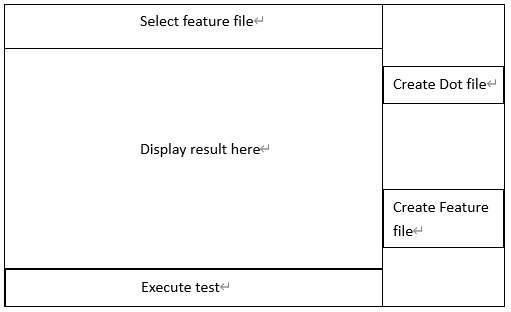
\includegraphics[width=10cm]{figures/mainMenu.png}\\
	\caption{Design concept for main menu.}
	\label{fig:figure4}
\end{figure}
\noindent 
To test model, first user will need to create a .dot file that define the relation of the parameters. By select the create .dot file option in the menu, the user will be bought to a screen that can edit what parameters is in the model. To make this function even more convenient, there should be a way to visualize the relation of the parameters. By visualize the relation of the parameter, user can use it as a reference to aid them in the process. User will also need to edit the relation between them, next screen will need to display the parameters the user previous entered. The user can select what a parameter is related to, and like the previous part, the interface will also have a visualization to assist user, below is a design concept for this part:

\begin{figure}[H]
	\centering
	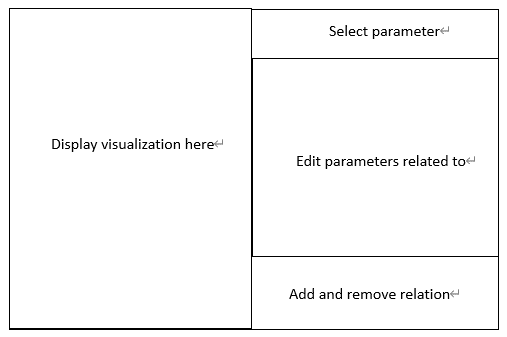
\includegraphics[width=10cm]{figures/editDot2.png}\\
	\caption{Part 2.Design concept for edit .dot function.}
	\label{fig:figure6}
\end{figure}
\noindent 
After edit the relation of parameter, user will need to edit some of the auto generated files to run the model and read the output, the purpose of these file is for Causcumber to execute the tested model and read the information provided by the model. This part assumed the user have certain level of knowledge in programming, that they have to ability to modify those files\\*\\*
When all the setup process is done, user can start creating feature file as test case, user can select the edit feature file function from the main screen edit it. This function will be structured in a way that is easy to navigate and mostly represent how the final feature file will look like. Since feature file are more complex compared to .dot file, there are more steps required to accomplished this process. \\*\\*
First, user need to define the parameters, parameter type and its value, this setup the tested parameter and their value. User will also need to define what parameter needs to be record. Below is a design concept for this part: 

\begin{figure}[H]
	\centering
	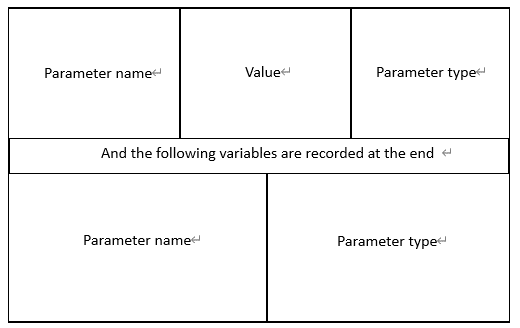
\includegraphics[width=10cm]{figures/editFeature1.png}\\
	\caption{Part 1.Design concept for edit .feature function.}
	\label{fig:figure7}
\end{figure}
\noindent 
Then, user will need to define edges for the parameters entered in the first part, this part should be similar to the previous edit .dot part to keep the consistence of the system, with some minor change.\\*\\*
Finally, user can start defining the scenarios. In scenarios, user can define a certain situation such as increase the value of a certain variable, and what the expect outcome of the system will be, visualization is also provide to assist user in the process. Below is a design concept for this part:

\begin{figure}[H]
	\centering
	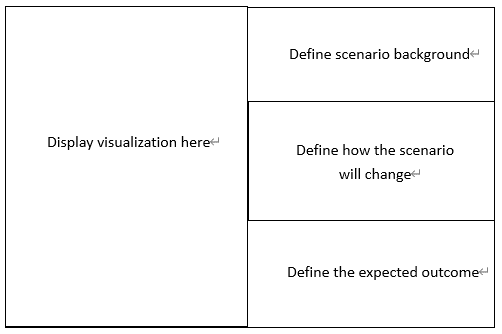
\includegraphics[width=10cm]{figures/editFeature2.png}\\
	\caption{Part 2.Design concept for edit .feature function.}
	\label{fig:figure8}
\end{figure}





